\section{Environment plug-in}

\subsection{Overview}

The architecture of the plug-in comes from
\cite{DeclarativeArchitecture}, to provide an intuitive way of
building an environment: by drawing features on a map. The most
difficult part in this approach is that intersecting features are
allowed and should give a result consistent with user expectations.

As a starting point, we focused on generating a height map, using the
concepts from \cite{FeatureTree}. It had the advantage of being able
to merge different environments (mountains, cities, ...) smoothly whenever they intersect, rather than using
the more convoluted conflict-resolution mechanism of
\cite{DeclarativeArchitecture}.

\bigskip

The basic unit managed by this plug-in is a \emph{feature}, which lies
in a certain area, has a certain height profile and knows how to
interact with the other features that may intersect it. From the
collection of all the features drawn on the map by the user, our
plug-in builds a tree encoding how to build the final height map by
successively merging sets of features together.  %TODO: mention models


%% Mettre un example de carte + rendu ici ?

\subsection{Features}
Features are individual ``areas''. Each feature contain several pieces of information:
\begin{itemize}
  \item The heightmap on it (the height of the terrain on every point of the feature).
  \item Models that can appear on the feature (trees, buildings, ...).
  \item How the feature interact with other features when intersecting
\end{itemize}
We now present some features we implemented.

\subsubsection{Mountains}

Our first implementation of the Mountain feature corresponded to what
is presented in \cite{FeatureTree}, where mountains are generated
procedurally. However, the 2D random functions we tried did not yield
satisfying results. That is why we switched to another version, where
we import at random a part of a heightmap taken from a website
\cite{terrain-party}. This website import the heightmaps through
satellite imaging.

\subsubsection{Roads}
Road are polylines with constant height. It means that a road is a succession of contiguous segments, and the height of the feature is the same constant everywhere on the road. 


\subsubsection{Vegetation (forests)}
Vegetation takes a model as input (as well as the polygonal shape). It duplicates this models randomly over the shape. The height is zero everywhere.

Last version allow to set a list of models for one forest instead of only one model.


\subsubsection{Cities}

We planned a feature that could generate cities, following a
three-step process. First, draw the street network. For this task we
chose to use the method of \cite{StreetTensors}, which provides a more
or less intuitive way for the user to control the output. Then, divide
each street-delimited block into parcels. We chose to follow the
approach of \cite{PGParcels}, which seemed to give realistic
results. Finally, put a building in each parcel. We did not look much
into that last part because using buildings of random height was
thought to be a reasonable approximation.

However, even the first step turned out to be challenging to
implement. The principle of the chosen method was to describe the
shape of the street network by a tensor field, mapping points to $2
\times 2$ matrices. It is described by a combination of basic fields
given by the user. The streets are then drawn as the stream lines of
the eigenvectors of the field. The main issue here was to represent
the street network under construction so that:
\begin{itemize}
  \item street drawing starts from points belonging to old streets and
satisfying certain constraints
  \item new intersections are correctly handled while drawing a street
  \item the right eigenvector is always chosen
\end{itemize} without having to reimplement the computation of
eigenvectors or the numerical approximation of a differential
equation.

%% On ne parle pas trop de ce qui allait pas là non ?


\subsection{Mixing Features}
Now we want to mix these features to be able to generate full environments.

For that, we first generate a \textit{FeatureTree}, to build a hierarchy of the different features. Using this tree, we generate a heightmap and list of models of the environment (a model is a 2D position on the map and a path to a 3D model). And with all these elements, we finally create the Blender 3D scene.

\begin{figure}[h]
  \begin{center}
    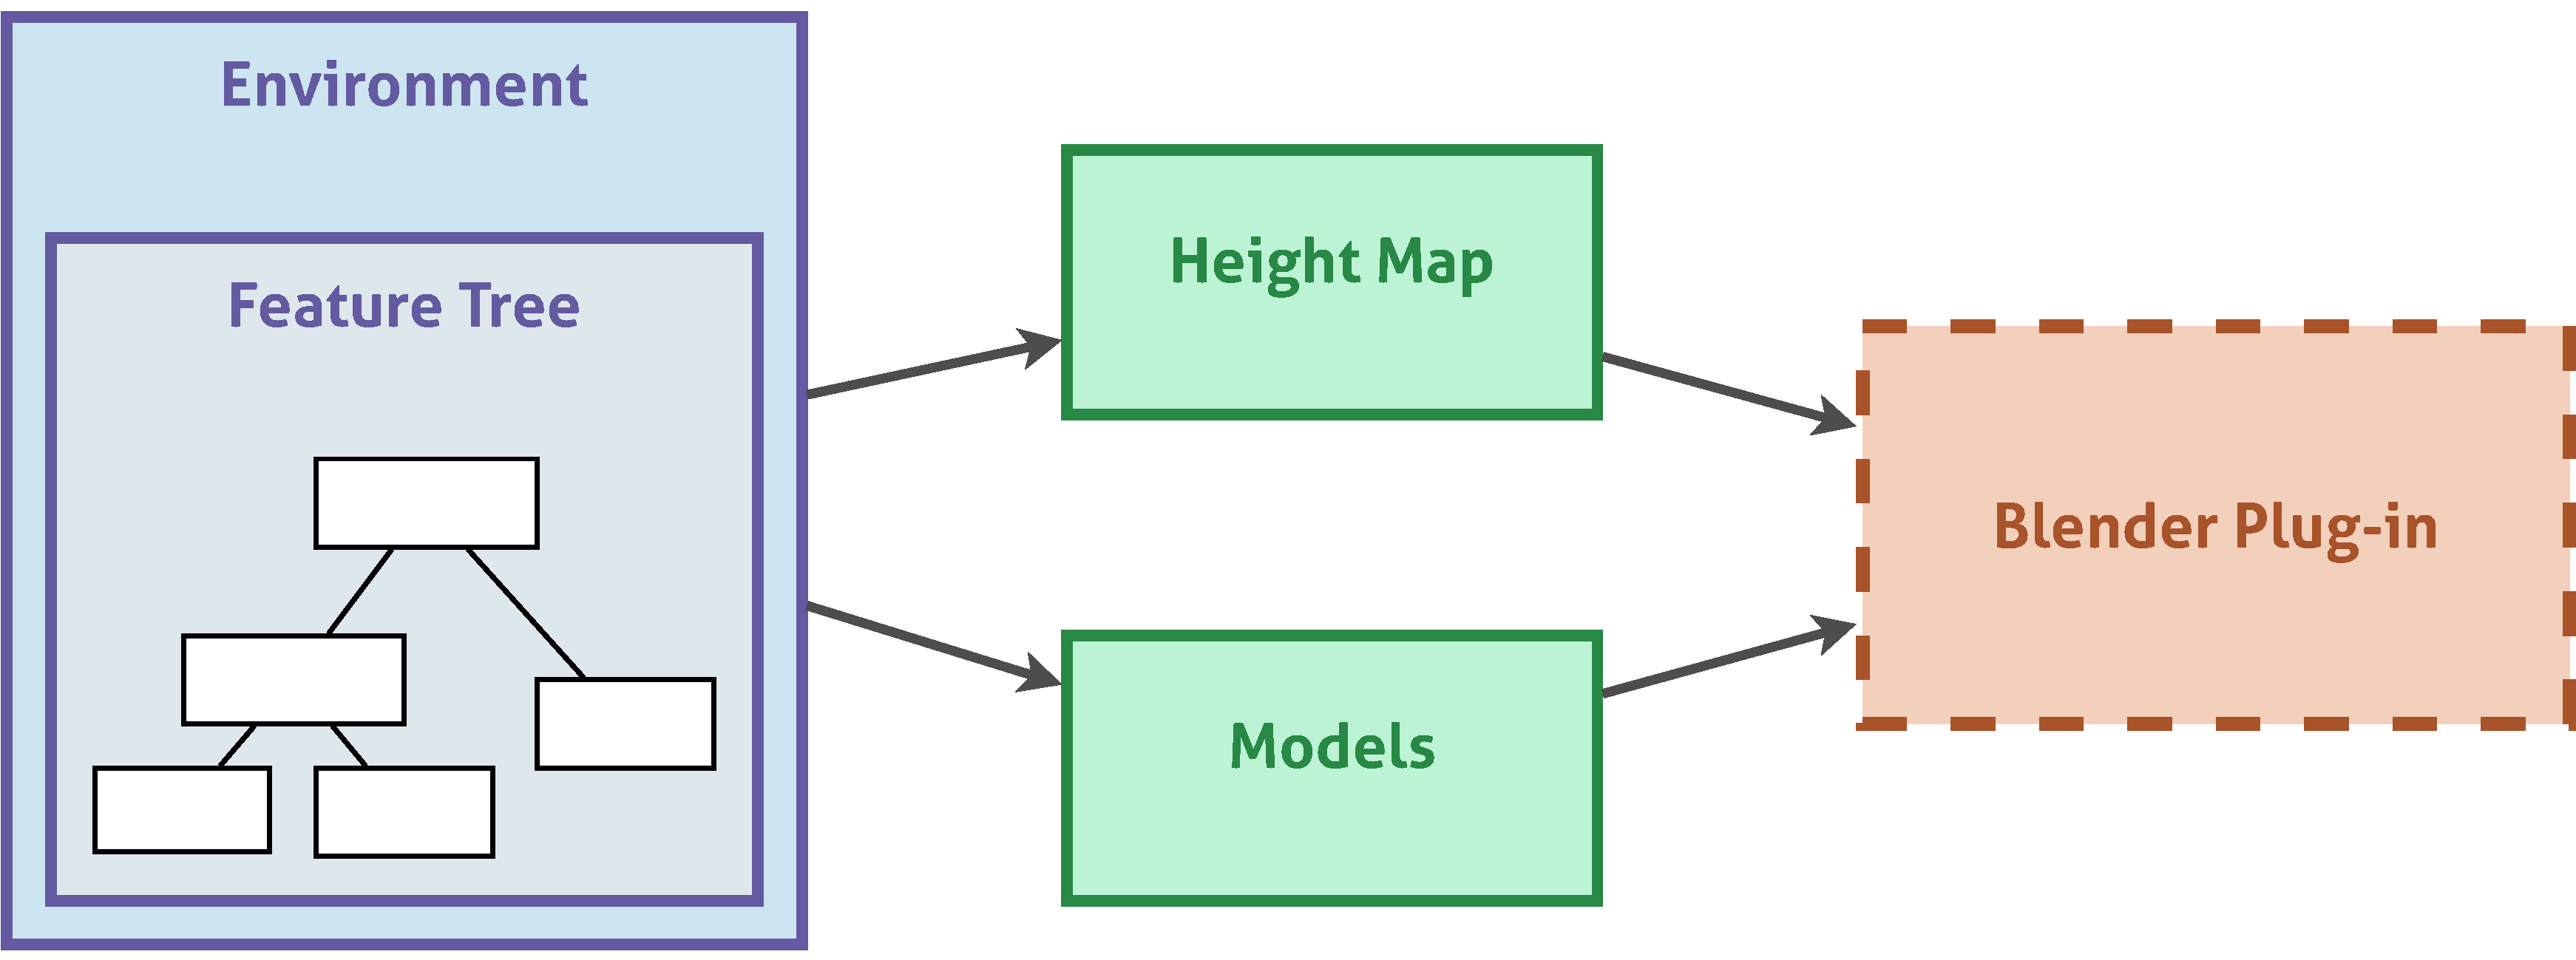
\includegraphics[width=10cm]{img/env_global.pdf}
    \caption{Organisation of the Environment plug-in}
    \label{fig:env_global}
  \end{center}
\end{figure}

This algorithm does everything without knowing what the feature are. Thus, it can mix any type of features. The user can define its own feature because the algorithm is general enough to handle any features.


\subsubsection{FeatureTree}
This data structure takes as input a list of features, and outputs a structured tree of the features, according how they are suppose to interact. 

The height of a point on the full map is just a recursive call of the height in the tree (see Fig.~\ref{fig:tree}).

\begin{figure}[h]
  \begin{center}
      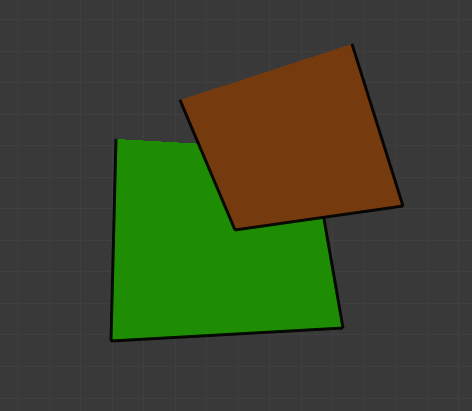
\includegraphics[width=4cm]{img/feature_2.png} ~
      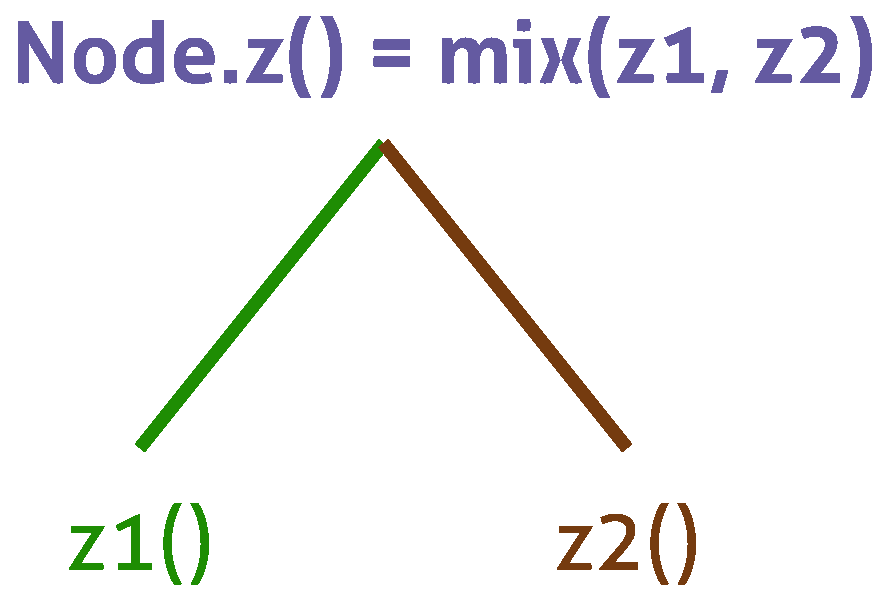
\includegraphics[width=4cm]{img/mix.pdf}
      \caption{Tree for height computation}
      \label{fig:tree}
   \end{center}
\end{figure}

Every feature has 3 different type of interaction with other features:
\begin{description}
  \item[Blend:] the intersection of the two features is the mean of the two features 
  (mix = $\frac{z1+z2}{2}$). This is what we use for mountains.
  \item[Replace:] the feature erase all features it intersects with (mix = z1). This interaction is used for lakes, and rivers.
  \item[Addition:] the feature adds it height to features lower in the tree (mix = $z1+z2$). This kind of interaction is used for forests and roads.
\end{description}
When two features intersects and have different fusion modes, the priority is as follows:\\
 Replace $>$ Addition $>$ Blend

The tree is generated by iterating over all feature intersections, and generating appropriated nodes for the 3 different possible interactions.
Thanks to the library \textit{Shapely}, geometric manipulation for generating intersections of polygons, were quite easy to code.

\subsubsection{Environment}
Now that the FeatureTree is generated, it is easy to generate the heightmap: for every pixel of the heightmap, compute the height of this points. Heights are then normalized and written into a png file.

For the models, we look at all models inserted by ``individuals'' features, and we add them to the global list of models, removing those which are ``erased'' by \textit{Replace} features. Then the height (z position) of every model is computed, thanks to the previous heightmap and the (x,y) position of every models.

\subsubsection{Interaction with Blender}
Now we have everything to create our environment!
The Blender plug-in uses previous data structures to generate a plane and applies to it the heightmap. It then import all models and insert them in the scene using their (x,y,z) position.

All parameters of the features and feature tree are modifiable via a graphical interface.


\subsection{Graphical User Interface (GUI)}

A picture of the interface is presented in
Fig.~\ref{fig:env-gui1}. Using the interface, the user can choose the
feature he wants to draw. He can then draw it using a pencil
integrated in Blender, drawing polygons here. After having completed
the drawing of the features, the user can ask for the generation of
the environment. It can then hide the polygons, and also modify
parameters that are feature-specific.

\begin{figure}[h]
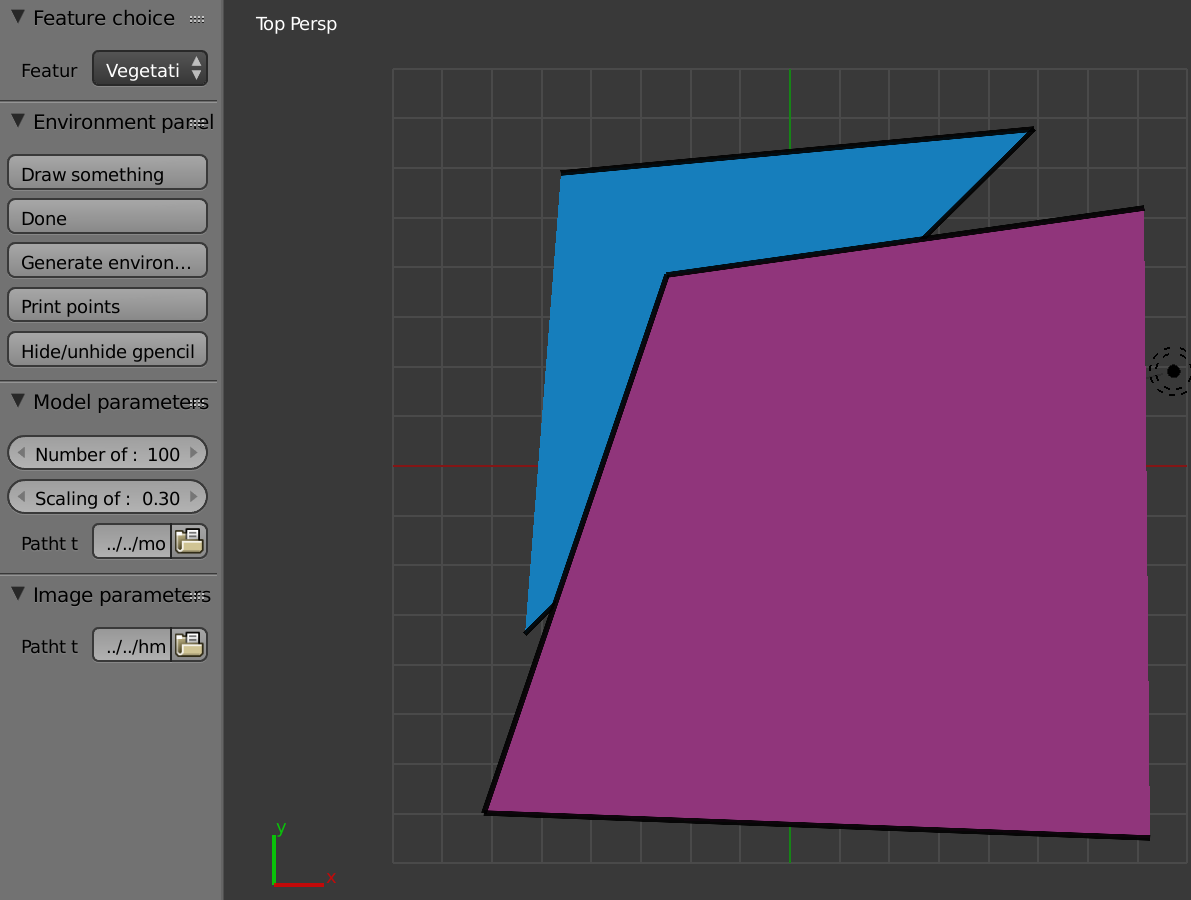
\includegraphics[width=\textwidth]{img/env_gui1.png}
\caption{GUI of the Environment plug-in, with two features (in blue
and magenta)}
\label{fig:env-gui1}
\end{figure}

%% Eventuellement : faire deux images, une du dessin des features, et
%% une de la génération ?
